\documentclass{book}

\usepackage[]{graphicx}

\title{Design Document}
\author{Jens Henninger \and Daniel Maier \and Paul Fink \and Florian Jennewein}
\date{\today}


\begin{document}
\frontmatter
\maketitle
\tableofcontents
\mainmatter
\part{Architectural Design}

\chapter{Introduction}
This architectural document describes the architecture of the desired system "Sojabohne" from different perspectives and in different levels of detail. All references to requirements are based on the system requirements of our requirements-document from 26.11.2015\footnote{https://moodle.uni-mainz.de/pluginfile.php/33185/assignsubmission\_file/submission\_files/8942/Abgabe\_Review\_Document.tar.gz}.
\chapter{External Layer}
Because there is no connection between our system and other ones, Sojabohne is set in a standalone-context(cf.Figure 2.1). \\\\\\\\
\begin{figure}[h]
\centering
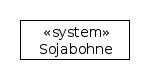
\includegraphics[width=3cm]{Context_Model.jpg}
\caption{Our system in standalone context :)}
\label{Fig. 1}
\end{figure}
\chapter{Structural Layer}
Obviously the most basic systemstructure is based on the Client-Server Pattern. That's because in this pattern, the server provides services, in our case mainly the appliance of data mining and machine learning algorithms on a user uploaded data. An user shall be able to access the result and the data itself from all over the world(if he has the required rights to do so) via the web application(cf. NFR017.0/NFR005.0). So we use the client-server-pattern, where the web application is the client and the server is the system, who executes the algorithms inclusive the database.\\\\\\\\
\begin{figure}[h]
\centering
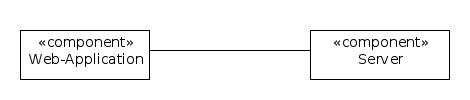
\includegraphics[width=9cm]{Client-Server.jpg}
\caption{Web-application as client; with the server.}
\label{Fig. 2}
\end{figure} 
\chapter{Used Patterns}
\chapter{Interaction Layer}
The following section attends to the interaction between the different aleready mentioned system components in different scenarios. The main task is the visualization of the data exchange with sequence-diagrams; without an exact definition of the called methods.
 
\end{document}

%%% Local Variables:
%%% mode: latex
%%% TeX-master: t
%%% End:
